Deep neural networks are famous for their obscurity. The interpretation of the results obtained using these techniques \tchanged{is more challenging than}
obtaining the results themselves. The difficulty of interpretation brews the suspiction that the neural network learns 
artifacts in the data that correlate with the target result. In this section we attempt to show, that our network 
learns relevant description of a protein structure and does not rely on small differences in submissions between prediction groups.

First, we analyse the regions of the structures that are responsible for the \tchanged{increase} in its score. The method we use was proposed 
by Selvaraju R. \cite{selvaraju2016grad}. The key idea of this technique is to propagate the gradient to a certain layer and take the sum of the 
activations of this layer weighted by the gradient. The weighted activation maps are then upscaled to the whole reception field of the network.
They indicate which parts of the input contributes the most to the gradient of the network output. In our case we chose the activations 
of the ReLU layer 10. The volumes of these activation maps are 25x25x25 which are the best tradeoff between interpretability and the coarsness 
of the maps. The example of the output is given on the Fig. \ref{Fig:GradCAMT0776}. Accoding to our scoring procedure we uniformly sample rotations 
and translations of a decoy. Here we follow the same procedure: we sample tranformations, obtain the activation maps, project them onto 
the atoms of the decoy. Afterwards, we average projected values and plot them using rainbow coloscheme (Fig. \ref{Fig:GradCAMT0776}). 
Figure \ref{Fig:GradCAMT0776_more} shows several examples of the decoys for the target T0776. 
The activations maps show, that the network enforces packing: the increase in the density 
around the well packed core is penalized. Surprisingly, we found that the activation maps, obtained in the abovementioned way, 
are mostly zero for the structures close to the native ones, despite that the information about gradients was not included in 
the training procedure. 

\begin{figure}[H]
    \centering
    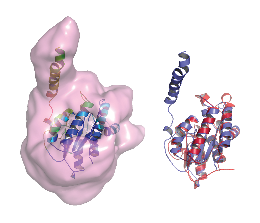
\includegraphics[width=0.5\linewidth]{Fig/FigT0776.eps}
    \caption{The scaled gradient weighted activation maps of the network (left). 
    This example shows the candidate structure Distill\_TS3 for 
    the target T0776. On the right side the native structure (red) is aligned to the candidate (blue). The left side shows the activation 
    map with the isodurface at the level two sigma (the maps were normalized). The values of the activation map at the coordinated of protein
    atoms are shown with the color from blue to red.}
    \label{Fig:GradCAMT0776}
\end{figure}

\begin{figure}[H]
    \centering
    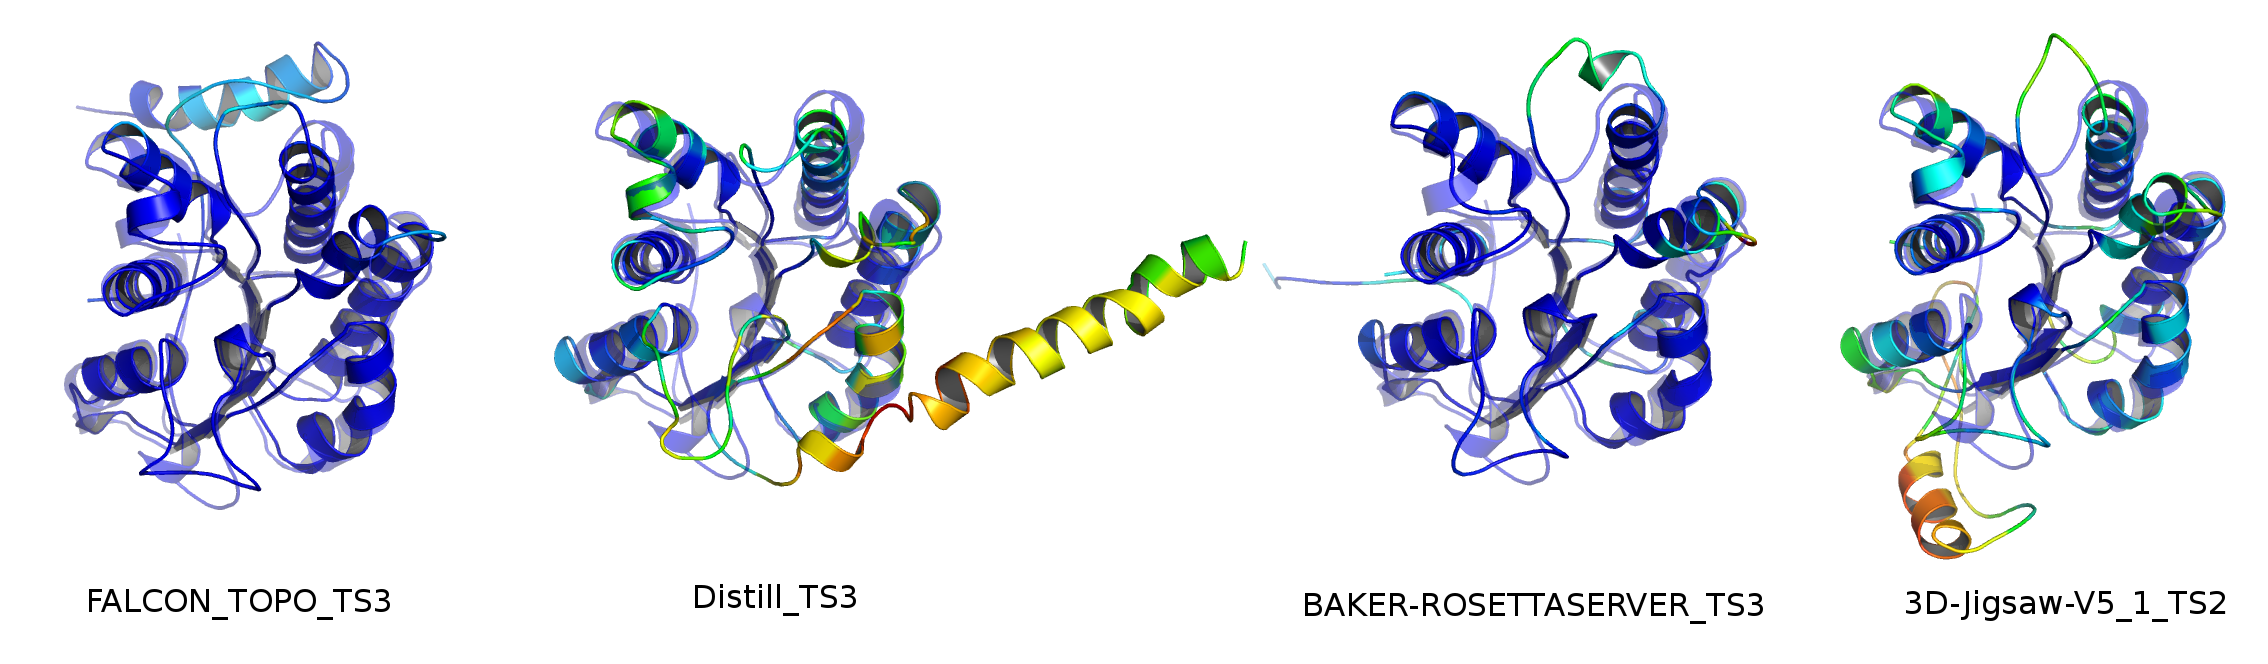
\includegraphics[width=\linewidth]{Fig/T0776.eps}
    \caption{The scaled gradient weighted activation maps of the network projected onto the atoms of the decoys. 
    Each decoy is aligned to the native structure (shown with the transparent cartoon).}
    \label{Fig:GradCAMT0776_more}
\end{figure}

To verify that the network we trained does not rely on artifacts in the data to rank decoys, we assessed the ranking on the dataset, designed 
by the 3DRobot algorithm \cite{deng20163drobot}. The decoys generated by this algorithm are 
uniformly distributed within RMSD range of $[0; 12\AA]$. They 
were optimized for the number of hydrogen bonds and compactness.
The absolute spearman R-coefficient averaged over all the structures in this benchmark was $0.85$, Spearman coefficient and Kendall tau were
0.83 and 0.64 respectively. The representative examples of scoring funnels are shown on the Fig \ref{Fig:3DRobotBenchmark}. 
We see, that the QA method we devised
in this work successfully ranks unrelated dataset, that has the same hyperparameters of the underlying decoys generator.

\begin{figure}[H]
    \centering
    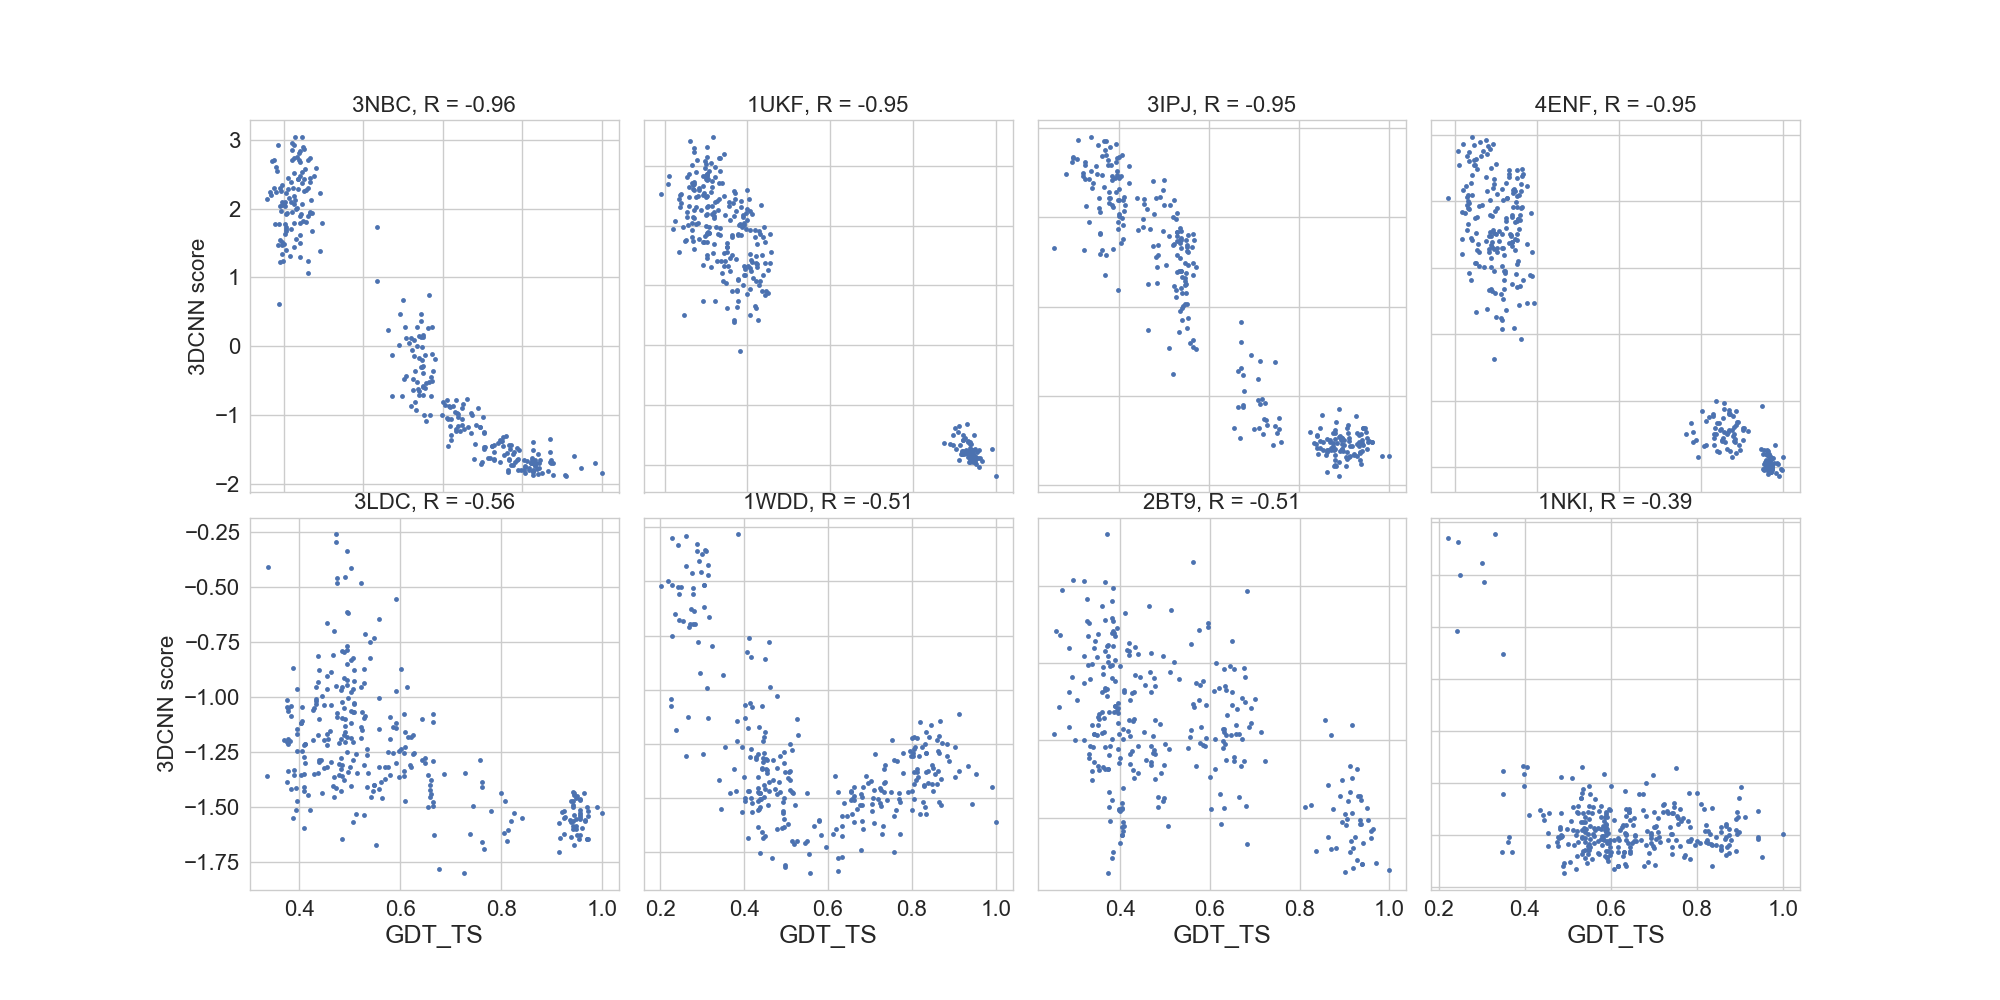
\includegraphics[width=\linewidth]{Fig/3DRobot_set_sFinal_funnels.eps}
    \caption{The scoring funnels of four best correlated targets and four least correlated targets in 3DRobot benchmark.}
    \label{Fig:3DRobotBenchmark}
\end{figure}